%background
\chapter{Chapter Title} 

%\label{ch:bg}

\section{Analysis}

To tackle the problem described in \hyperref[subsec:problem-statement]{Section \ref*{subsec:problem-statement}}, we will use Reinforcement learning with Deep Learning to automatically learn evaluation functions by playing games by itself. Unlike other approaches that need a very large dataset, this approach will try to learn to play games without any domain knowledge (no dataset will be used). This is a promising approach for creating game-playing algorithms for playing other two-player games of perfect information.

%%%%%%%%%%%%%%%%%%%%%%%%%%%%%%%%%%%%%%%%%%%
\subsection{Data Exploration and Visualization}

\subsubsection{Coaster Racer Game environment}

The browser screenshot as shown in Figure 2 is both for the user and the AI Game Bot. Namely, that is the raw vision of the Game Bot which apparently contains lots of pixels useless for deciding the steering. For more efficient and faster computing, some preprocessing procedures would be done before we throw the image data into a deep learning model, which will be described in later paragraph.

\begin{figure}[h]
\centering
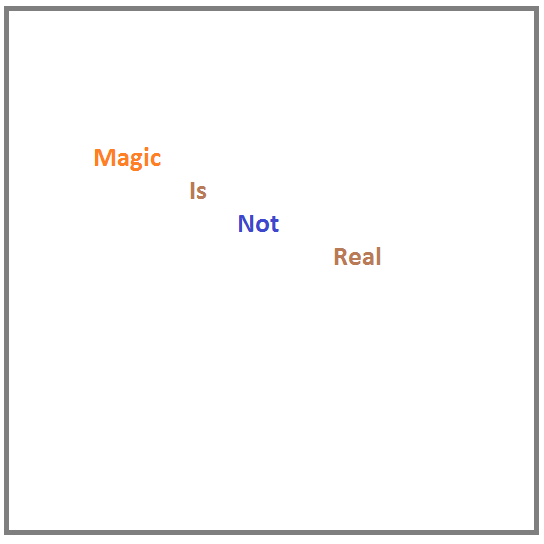
\includegraphics[width=0.5\textwidth]{figs/magic}
\caption{A browser screenshot of Coaster Racer Game.}
\end{figure}

\subsubsection{States}

For the purposes of winning the game, the state of the game at time t is simply the pixel array of the game screen at that particular time. I experimented with using only a cropped version of the game screen that contained the view of the driver. In order to avoid unnecessary computation and memory usage, we downsample this image. By reducing the size of each state, this allows us to fit more training examples in our replay history without running out of memory, which is a crucial component of the experience replay technique we used. In addition, with lower-dimensional input, our network requires fewer matrix multiplications and fewer parameters in the fully connected layers, greatly improving speed.

\begin{itemize}
		
	\item State Space: {Preprocessed screenshots of the browser loading the game}

\end{itemize}

\subsubsection{Actions}

Coaster Racer Flash Game is a typical car racing game which is simply controlled by moving forward, left turn and right turn. With this simple setting, we only only an action space of three actions, namely, moving forward, left turn and right turn.

\begin{itemize}
	
	\item Action Space: {Move Forward action, Turn Left action, Turn Right action}

\end{itemize}

\subsubsection{Rewards}

Rewards are primarily based off of the game score. From the perspective of human player, we judge a good player or not by how the driving behavior is close to real and safe case. While for a Game Bot, it only cares about the score. For this specific game, Coaster Racer Game, it unreasonably encourages a dangerous driving behavior. For example, when the car hits a traffic cone it gets 1000 reward, even if the price of hitting a cone is falling down the road. There is no punishment for falling down the road.

An ideal reward function would encourage the car to stay in the middle of the road and to try not to hitting other cars and guard bars. Here I simply cancel the one time 1000 score reward. But there is still room to fine tune the function in the future.

%%%%%%%%%%%%%%%%%%%%%%%%%%%%%%%%%%%%%%%%%%%
\subsection{Algorithms and Techniques}

\subsubsection{Overal Representation}

\begin{figure}[h]
\centering
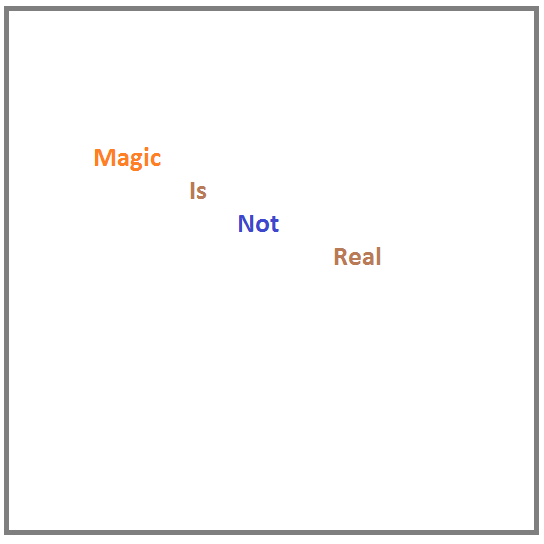
\includegraphics[width=0.5\textwidth]{figs/magic}
\caption{A flowchart of training the Coaster Racer Game Bot.}
\end{figure}

An overall representation of how the different components relate during a play evaluation, centered around the deep Q-network for playing, the main decision component is shown in Figure 3. Each game screen is resized to a desaturated pixels image, and if you might be wondering why each state is a sequence of four game screens instead of one, that is because the agent's history is used for better motion perception. Achieving this requires a sequence of preprocessed images to be stacked in channels (like you would stack RGB channels on a colored image) and fed to the network.

%%%%%%%%%%%%%%%%%%%%%%%%%%%%%%%%%%%%%%%%%%%%%
\subsubsection{Deep Neural Network}
%%%%%%%%%%%%%%%%%%%%%%%%%%%%%%%%%%%%%%%%%%%%%

Convolutional Neural Networks, or CNNs, are a special type of neural network that has a known grid-like topology. Like most other neural networks they are trained with a variant of the back-propagation algorithm. CNN's strength is pattern recognition directly from pixels of images with minimal processing. We use a convolutional network as a function mapping the preprocessed images to Q values, since the actions are highly based on what would be seen as pixel matrix.

\begin{itemize}

	\item \textbf{DeepMind's Deep Q Network}
	
	\begin{figure}[h]
	\centering
	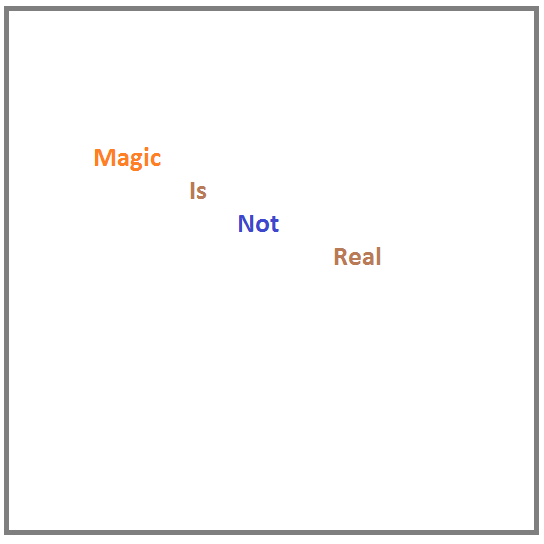
\includegraphics[width=0.5\textwidth]{figs/magic}
	\caption{Deep Neural Network model from DeepMind paper.}
	\end{figure}
	
	The network's architecture that I firstly used is essentially the same used by DeepMind, except for the first convolutional neural network's input (80x80x4 instead of 84x84x4, to account for the different input sizes) and the linear layer's output (3 instead of 18, to account for the different number of actions available).
	
	\item \textbf{LeNet-5.}
	
	\begin{figure}[h]
	\centering
	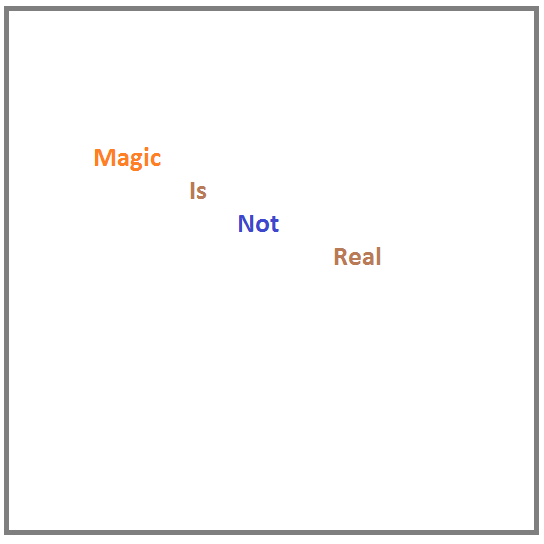
\includegraphics[width=0.5\textwidth]{figs/magic}
	\caption{LeNet-5.}
	\end{figure}
	
	For an image classification problem, there are several mature models other than the one above such as LeNet, VGG, Inception and Xception. I then tried a LeNet-5 model here and expected it to perform better than the DeepMind one for predicting actions. LeNet is deeper than the DeepMind one to grasp more features and has some dropout layers to avoid overfitting. In practice, it shows an advantage especially on predicting turning actions.
	
\end{itemize}

%%%%%%%%%%%%%%%%%%%%%%%%%%
\subsubsection{Q-learning}
%%%%%%%%%%%%%%%%%%%%%%%%%%

One of the most basic and popular methods to estimate action-value functions is the \emph{Q-learning} algorithm. It is model-free online off-policy algorithm, whose main strength is that it is able to compare the expected utility of the available actions without requiring a model of the environment. Q-learning works by learning an action-value function that gives the expected utility of taking a given action in a given state and following a fixed policy thereafter.

A value function estimates what is good for an agent over the long run. It estimates the expected outcome from any given state, by summarizing the total amount of reward that an agent can expect to accumulate into a single number. Value functions are defined for particular policies.

The \emph{state value function} (or V-function), is the expected return when starting in state $s$ and following policy $\pi$ thereafter~\citep{Sutton1998RL},
%
\begin{equation}
V^\pi(s) = \mathbb{E}_\pi \left[R_t | s_t = s \right]
\end{equation}

The \emph{action value function} (or Q-function), is the expected return after selecting action $a$ in state $s$ and then following policy $\pi$,
%
\begin{equation}
Q^\pi(s,a) = \mathbb{E}_\pi \left[ R_t | s_t = s, a_t = a \right]
\end{equation}

The \emph{optimal value function} is the unique value function that maximises the value of every state, or state-action pair,
%
\begin{eqnarray}
Q^*(s,a) & = & \max\limits_\pi Q^\pi(s,a), \forall s \in \mathcal{S}, a \in \mathcal{A}
\end{eqnarray}

An \emph{optimal policy} $\pi^*(s,a)$ is a policy that maximises the action value function from every state in the MDP,
%
\begin{equation}
    \pi^*(s,a) = \argmax_\pi Q^\pi(s, a)
\end{equation}

The update rule uses action-values and a built-in max-operator over the action-values of the next state in order to update $Q(s_t, a_t)$ as follows,

\begin{equation}
Q(s_t,a_t) \gets Q(s_t,a_t) + \alpha \left[r_{t+1} + \gamma \max_a Q(s_{t+1},a) - Q(s_t,a_t)\right]
\end{equation}

The agent makes a step in the environment from state $s_t$ to $s_{t+1}$ using action $a_t$ while receiving reward $r_t$. The update takes place on the action-value $a_t$ in the state $s_t$ from which this action was executed. This version of Q-learning works well for tasks with a small a state-space, since it uses arrays or tables with one entry for each state-action pair.

In this project the policy is using the \textbf{$\epsilon$-greedy} policy:

\begin{itemize}

    \item \textbf{$\epsilon$-greedy.} Selects the best action for a proportion
        $1 - \epsilon$ of the trials, and another action is randomly selected (with
        uniform probability) for a proportion,
        
        \begin{equation}
            \pi_{\epsilon}(s) = \left\{
             \begin{array}{lr}
                 \pi_{\textrm{rand}}(s,a) & \text{if } rand() < \epsilon\\
                 \pi_{\textrm{greedy}}(s,a) & \text{otherwise}
             \end{array}
           \right.
        \end{equation}

        where $\epsilon \in [0, 1]$ and $rand()$ returns a random number from a uniform distribution $\in [0, 1]$.

\end{itemize}

%%%%%%%%%%%%%%%%%%%%%%%%%%%%%%%%%%%%%%%%%%%
\subsection{Benchmark}

This benchmark consists in playing against an agent that takes uniformly random moves. This is the most basic benchmark, but first we have to be sure that our learned evaluation function can play better than a random agent before moving into a harder benchmark. Also, this will help us to detect bugs in the code and algorithms: if a learned value function does not play significantly better than a random agent, is not learning. The idea is to test against this benchmark using Alpha-beta pruning at 1, 2 and 4-ply search.

%%%%%%%%%%%%%%%%%%%%%%%%%%%%%%%%%%%%%%%%%%%%%%%%%%%%%%%%%%%%%%%%%%%%%%%%%%%%%%%%%%%%%%%%%%%%%%%%%%%%





%\bibliographystyle{plainnat}				%Uncomment this if you want a bibliography on each chapter
%\markright{\textit{Bibliography}}
%\renewcommand{\chaptername}{}
%\bibliography{my_references}

%\vfill

